% Options for packages loaded elsewhere
\PassOptionsToPackage{unicode}{hyperref}
\PassOptionsToPackage{hyphens}{url}
%
\documentclass[
]{article}
\usepackage{lmodern}
\usepackage{amssymb,amsmath}
\usepackage{ifxetex,ifluatex}
\ifnum 0\ifxetex 1\fi\ifluatex 1\fi=0 % if pdftex
  \usepackage[T1]{fontenc}
  \usepackage[utf8]{inputenc}
  \usepackage{textcomp} % provide euro and other symbols
\else % if luatex or xetex
  \usepackage{unicode-math}
  \defaultfontfeatures{Scale=MatchLowercase}
  \defaultfontfeatures[\rmfamily]{Ligatures=TeX,Scale=1}
\fi
% Use upquote if available, for straight quotes in verbatim environments
\IfFileExists{upquote.sty}{\usepackage{upquote}}{}
\IfFileExists{microtype.sty}{% use microtype if available
  \usepackage[]{microtype}
  \UseMicrotypeSet[protrusion]{basicmath} % disable protrusion for tt fonts
}{}
\makeatletter
\@ifundefined{KOMAClassName}{% if non-KOMA class
  \IfFileExists{parskip.sty}{%
    \usepackage{parskip}
  }{% else
    \setlength{\parindent}{0pt}
    \setlength{\parskip}{6pt plus 2pt minus 1pt}}
}{% if KOMA class
  \KOMAoptions{parskip=half}}
\makeatother
\usepackage{xcolor}
\IfFileExists{xurl.sty}{\usepackage{xurl}}{} % add URL line breaks if available
\IfFileExists{bookmark.sty}{\usepackage{bookmark}}{\usepackage{hyperref}}
\hypersetup{
  hidelinks,
  pdfcreator={LaTeX via pandoc}}
\urlstyle{same} % disable monospaced font for URLs
\usepackage{graphicx}
\makeatletter
\def\maxwidth{\ifdim\Gin@nat@width>\linewidth\linewidth\else\Gin@nat@width\fi}
\def\maxheight{\ifdim\Gin@nat@height>\textheight\textheight\else\Gin@nat@height\fi}
\makeatother
% Scale images if necessary, so that they will not overflow the page
% margins by default, and it is still possible to overwrite the defaults
% using explicit options in \includegraphics[width, height, ...]{}
\setkeys{Gin}{width=\maxwidth,height=\maxheight,keepaspectratio}
% Set default figure placement to htbp
\makeatletter
\def\fps@figure{htbp}
\makeatother
\setlength{\emergencystretch}{3em} % prevent overfull lines
\providecommand{\tightlist}{%
  \setlength{\itemsep}{0pt}\setlength{\parskip}{0pt}}
\setcounter{secnumdepth}{-\maxdimen} % remove section numbering
\ifluatex
  \usepackage{selnolig}  % disable illegal ligatures
\fi
\newlength{\cslhangindent}
\setlength{\cslhangindent}{1.5em}
\newenvironment{cslreferences}%
  {\setlength{\parindent}{0pt}%
  \everypar{\setlength{\hangindent}{\cslhangindent}}\ignorespaces}%
  {\par}

\author{}
\date{}

\begin{document}

\newcommand{\matr}[1]\textbf

\{\#1\}

\newcommand{\vect}[1]{\vec{#1}}

\hypertarget{to-my-dear-supervisors}{%
\section{To my dear supervisors}\label{to-my-dear-supervisors}}

Dear Professor Likos! Dear Dr.~Bianchi! Dear Professor Kahl!

I want to thank Professor Kahl for taking over the duty of supervising
my bachelor's thesis. I'm very relieved that (hopefully) the
administrative part has been taken care of. Dr.~Bianchi, thank you very
much again for organising everything.

A quick recap: This is the format I've chosen to report my progress.
I'll periodically send a report that is generated by jupyter notebook (a
science \& analysis environment for python). The notebook is here for
writing part of my thesis, as well as analyzing the data. The code is
written in C++. So please don't worry if not everything looks good yet -
the formatting, and improving the citation style as well as other things
will be done later, when the bachelor's has mostly been finished.

Last time I implemented the streaming step and did some work on random
generators, as well as finding my way into C++ again. It has been quite
some time and I'm happy to report some progress.

This time the MPCD barebones should be completely working (streaming +
collision + gridshift). Work was done on parallelizing the code (far too
much), but this has been scrapped for now. Additionally, I've written a
lot of analyzing code in python that will be there to generate some
hopefully interesting plots once everything has been implemented. The
code was tested, in my opinion, quite a lot, and I think there should be
no issues. But if you find anything that looks suspicious from this
report, just tell me right away.

Please stay in good health. Yours,

Chris

\hypertarget{mpcd-simulation-of-polymers-in-solution}{%
\section{MPCD simulation of polymers in
solution}\label{mpcd-simulation-of-polymers-in-solution}}

This notebook will serve as the documentation of our efforts and results
for my Bachelor's Thesis. The goal of this thesis will be the study of
short/long-chained polymers in a liquid thats flowing around obstacles.
The liquid will be simulated with MPCD, or ``Multi Particle Collision
Dynamics''.

I chose the language C++ for its familiar object-oriented nature and its
proven execution-time. Output of the simulation will mostly be analysed
in Python, specifically with Jupyter Notebook for a blend of beautiful
visualizations and convenience. For simplification, the situation will
be studied in 2D. The situation we specifically discussed is shown
below.

\begin{figure}
\centering
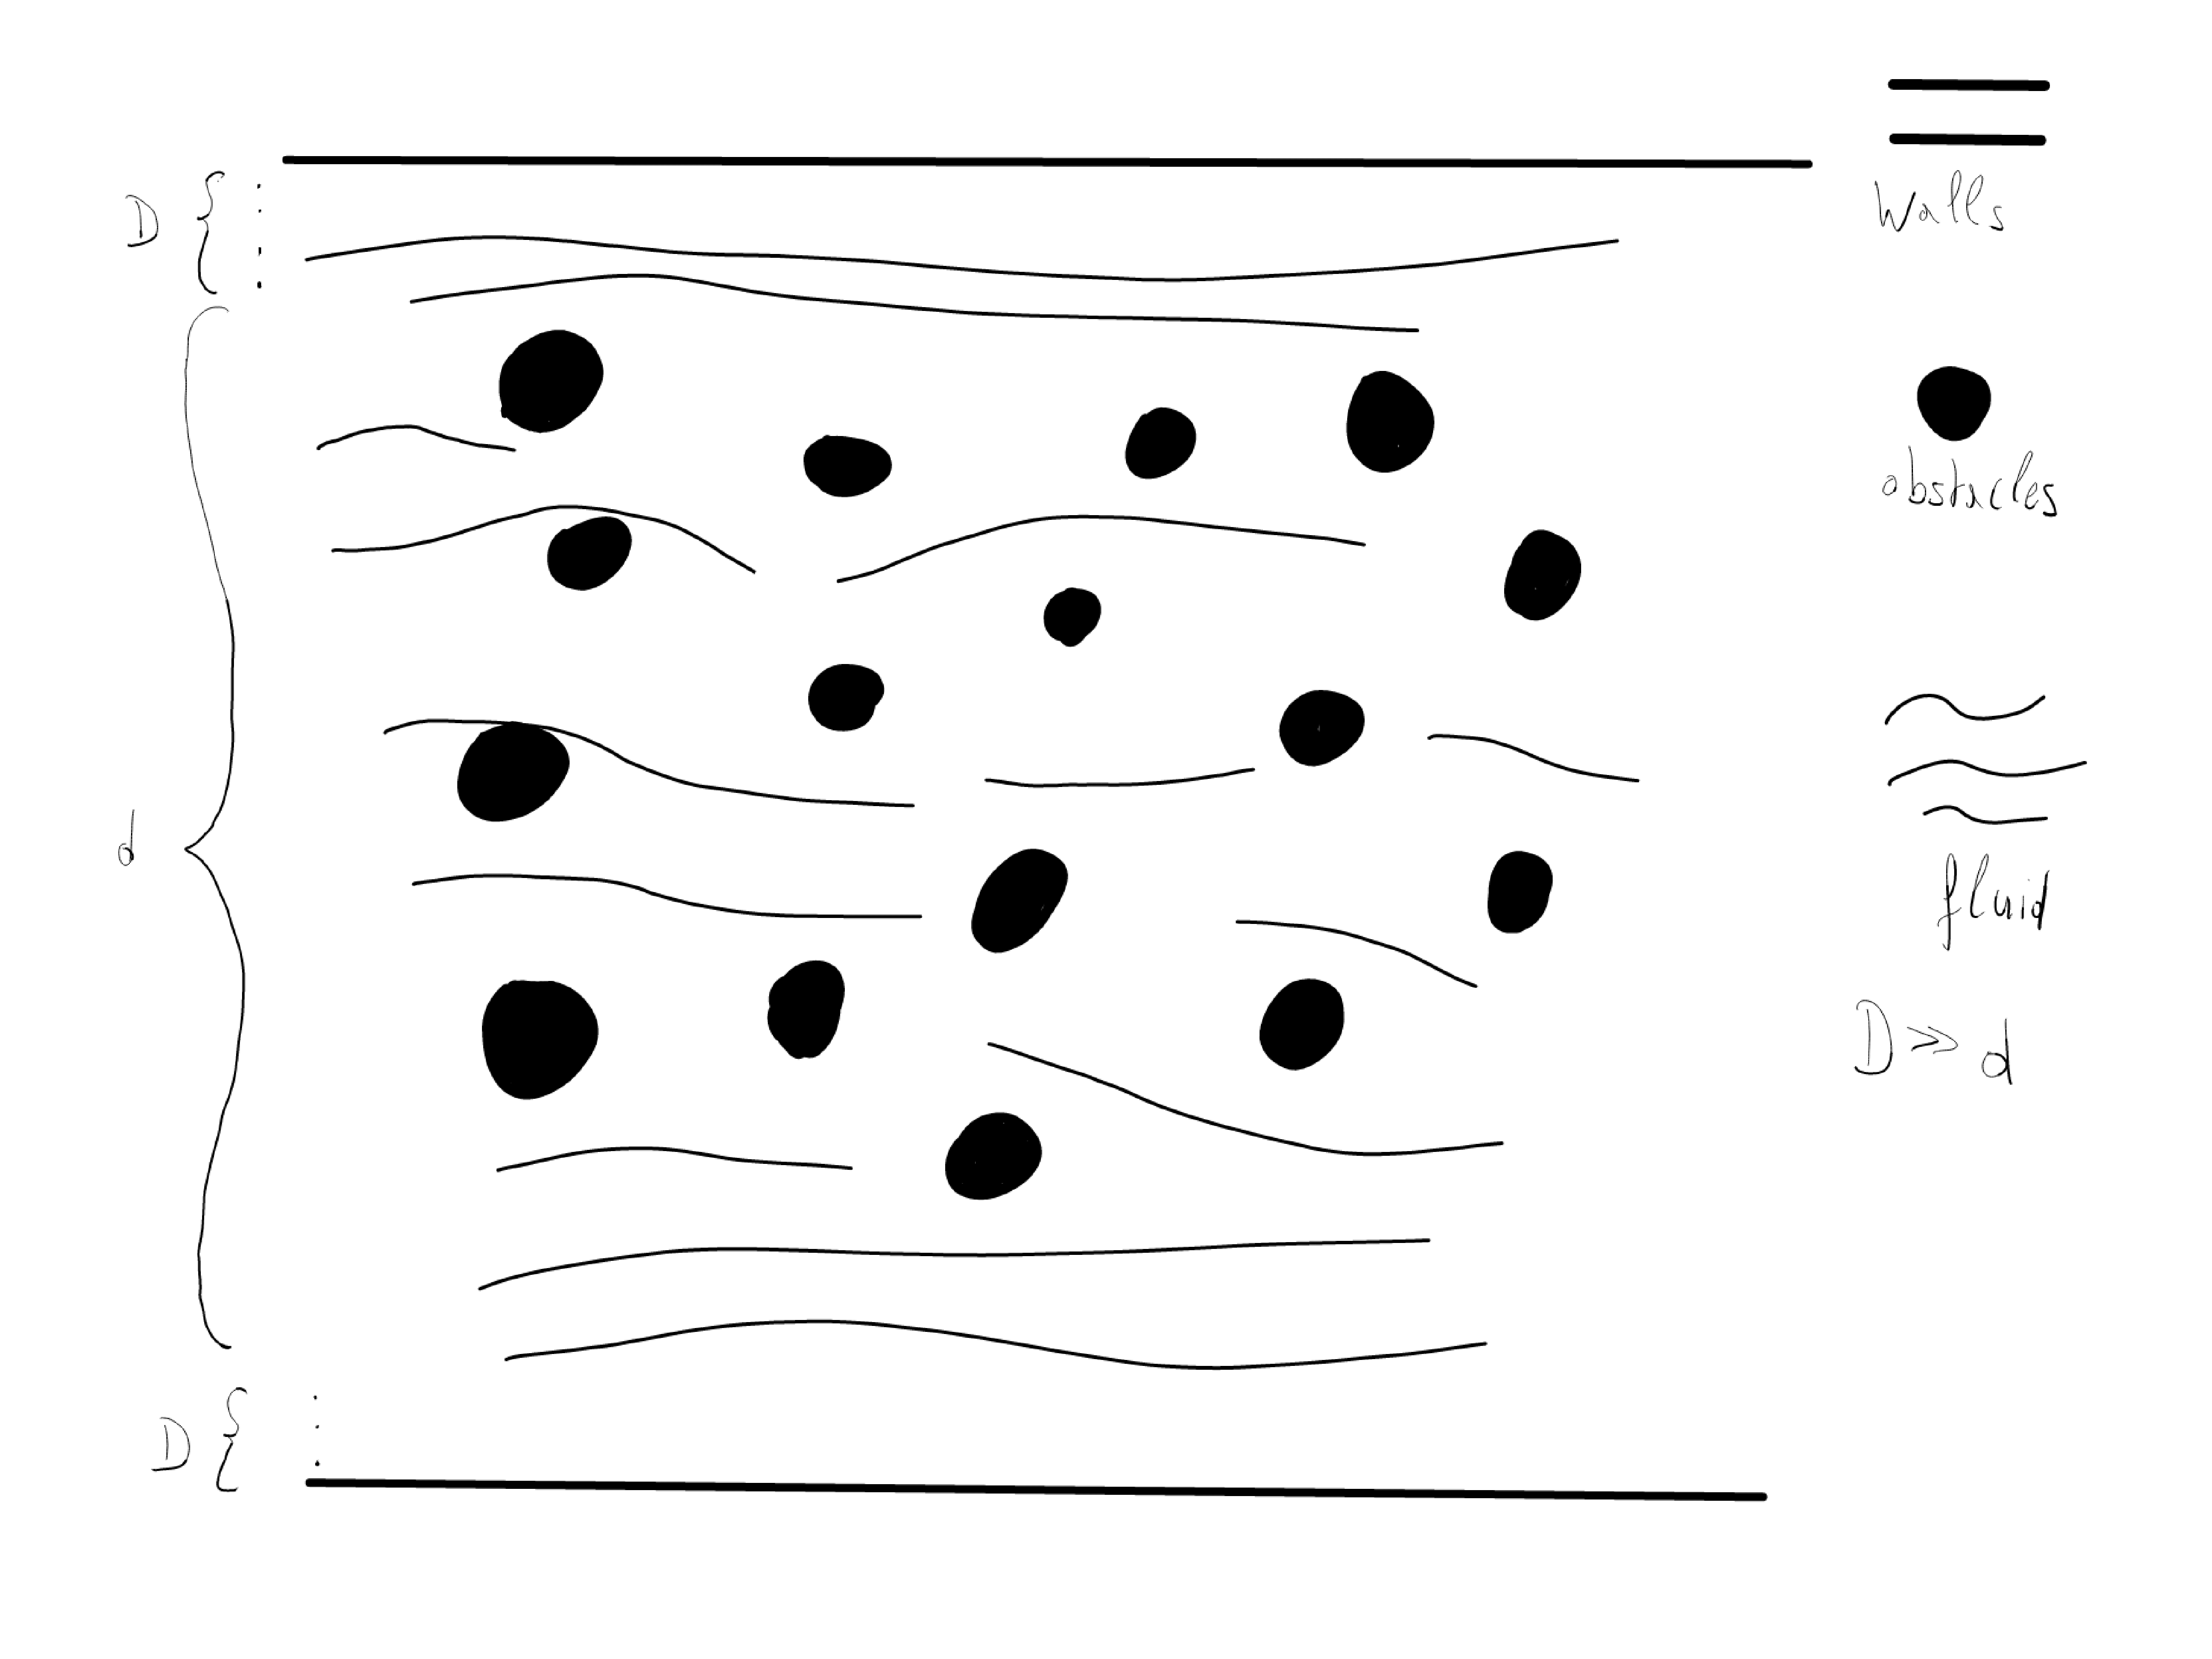
\includegraphics{Assets/MPCD_Situation.png}
\caption{Situation}
\end{figure}

\hypertarget{discussed-questions}{%
\section{Discussed questions}\label{discussed-questions}}

Are there other people I can contact for the programming/implementation
details? - \emph{Max Liebetreu, Andreas Zöddl}

How do I model the obstacles?, the walls? = the same? Many particles,
large molecules? circles? - \emph{Stick boundary conditions: velocity
gets flipped when colliding. Also: virtual particles for cell partially
filled by wall. Interaction with cylindrical obstacles is explained in
Arash's paper.}

How should I initialize the velocities? How large can they be without
distorting the simulation? - \emph{Maxwell Boltzmann with \(2/2 k_B T\)
(2D)}

If particles drift too far out of bounds, should they be destroyed, and
should then new ones be created to keep the number constant? In other
words, should there be a particle source? - \emph{Yes. The situation is
now fixed from 100 - 400 : 20 - 50 aspect ratio. When particles go out
of those bounds, they are ``teleported'' to the other side. This means
that it loops around, as if it was a ring, instead of a 2d pipe.}

How can I test if my simulation is right? See if some parameter can be
tuned to one of an experiment? How should we go about this? - \emph{See
if we get parabolic velocity profile for the 2d situation, after walls
have been added. Also check conservation of energy.}

Will we go to 3D? - \emph{For the Bachelor's, we will keep it 2D.}

\hypertarget{open-questions}{%
\section{Open Questions}\label{open-questions}}

On what order should \(D >> d\) in the drawing be? (see above) -
\emph{Still open.}

Half discussed: How large can the timestep be? - \emph{The timestep will
be a function of the other parameters. In Arash's paper, a unit of time
\(\tau = \sqrt{\frac{m a^2}{k_B T}}\) was chosen and from this somehow a
timestep was derived. For now, I'll take the same unit of time and make
the MPCD timestep 1/10 of that (just like Arash).} - Is that okay?

How should I choose the units, e.g.~mass, Temperature? (In Arash's paper
f.ex., T=1 was chosen) At the time I'm working with the mass of
H2O{[}kg{]} and Body Temperature{[}K{]}. - \emph{Still open.}

https://en.wikipedia.org/wiki/Hagen\%E2\%80\%93Poiseuille\_equation

Does the equation for pressure difference hold?

In standard fluid-kinetics notation:{[}5{]}{[}6{]}{[}7{]}

\{\displaystyle \Delta p=\{\frac {8\mu LQ}{\pi R^{4}}\}=\{\frac {8\pi \mu LQ}{A^{2}}\}\}\{\displaystyle \Delta p=\{\frac {8\mu LQ}{\pi R^{4}}\}=\{\frac {8\pi \mu LQ}{A^{2}}\}\}
where:

The ratio of length to radius of a pipe should be greater than one
forty-eighth of the Reynolds number for the Hagen--Poiseuille law to be
valid.{[}9{]} If the pipe is too short, the Hagen--Poiseuille equation
may result in unphysically high flow rates; the flow is bounded by
Bernoulli's principle, under less restrictive conditions, by

\{\displaystyle \Delta p=\{\frac {1}{2}\}\rho v\_\{\text{max}\}\textsuperscript{\{2\}=\{\frac {1}{2}\}\rho \left(\{\frac {Q_{\max }{}}{\pi R^{2}}\}\right)}\{2\},,,\rightarrow ,,,Q\_\{\max \}\{\}=\pi R\textsuperscript{\{2\}\{\sqrt {\frac {2\Delta p}{\rho }}\},\}\{\displaystyle \Delta p=\{\frac {1}{2}\}\rho v\_\{\text{max}\}}\{2\}=\{\frac {1}{2}\}\rho \left(\{\frac {Q_{\max }{}}{\pi R^{2}}\}\right)\textsuperscript{\{2\},,,\rightarrow ,,,Q\_\{\max \}\{\}=\pi R}\{2\}\{\sqrt {\frac {2\Delta p}{\rho }}\},\}
because it's impossible to have less-than-zero (absolute) pressure (not
to be confused with gauge pressure) in an incompressible flow.

\hypertarget{next-steps}{%
\section{Next Steps}\label{next-steps}}

\begin{enumerate}
\def\labelenumi{\arabic{enumi}.}
\tightlist
\item
  \_Check the conservation of energy, momentum, do the grid shift or the
  wall + particles + obstacles shift. - \_Done.\_\_
\item
  Constant Force that pull the particles in +x direction + Gamma cell
  level thermostat
\item
  Implement Wall logic, check if we get a parabolic flow profile.
\item
  Implement obstacle logic.
\item
  Polymers MD?
\end{enumerate}

\hypertarget{introduction}{%
\section{Introduction}\label{introduction}}

Multiparticle collision dynamics (MPCD), also known as Stochastic
Rotation Dynamics (SRD)(Gompper et al., 2009) is a technique originally
introduced to study the dynamics of complex fluids such as polymers in
solution. Besides MPCD, there exist other mesoscopic models that have
been constructed for this purpose, such as Langevin, Direct Simulation
Monte Carlo and lattice Boltzmann methods.(Malevanets \& Kapral, 1999)
We only concern ourselves with the application of MPCD, it follows that
any comparison between methods are out of the scope of this thesis.

The MPCD technique models the fluid using particles, their positions and
velocities are treated as continuous variables. The system is divided up
into cells that have no restriction on the number of particles, each of
the cells is part of a regular lattice. The dynamics is split into two
parts: Particle streaming and multiparticle collision dynamics. Particle
streaming is treated exactly for each particle in the system, while the
collision step is approximated on a cell level. The multiparticle
collision dynamics conserves mass, momentum and energy and leads to the
correct hydrodynamical equations.(Malevanets \& Kapral, 1999) The
streaming and collision step are described in more detail in (TODO:
section numbering).

\hypertarget{the-mpcd-algorithm}{%
\section{The MPCD algorithm}\label{the-mpcd-algorithm}}

The system we are modelling consists of \(N\) particles with mass \(m\),
continuous position \(\vec{r_{i}}\) and velocity \(\vec{v_{i}}\), where
\(i \in \{1, 2, \dots, N\}\). One timestep \(\Delta t\) shall correspond
to having calculated all the new particle positions and velocities in
the streaming and collision steps, respectively. For each of the \(N\)
particles, the streaming and collision steps are applied, and this
pattern is repeated until the wanted number of timesteps have elapsed.

\hypertarget{the-streaming-step}{%
\subsection{The streaming step}\label{the-streaming-step}}

The streaming step is very straightforward. The particle positions are
simply updated according to

\begin{equation}
\vec{r_{i}} \rightarrow \vec{r_{i}} + \Delta t \cdot \vec{v_{i}}\textrm{,}
\end{equation}

where \(\Delta t\) is a small time interval.(Gompper et al.,
2009)(Malevanets \& Kapral, 1999)

\hypertarget{the-collision-step}{%
\subsection{The collision step}\label{the-collision-step}}

The collision step is somewhat more complicated. It involves the mean
velocity of all particles in a particular cell, \(\vec{V_c}\), the
velocity of the particle \(i\), \(\vec{v_i}\), and a rotation matrix
\(\textbf(\alpha)\). The vector \(\vec{v_i}\) is rotated relative to the
mean velocity \(\vec{V_c}\) of all particles in cell \(c\), cell \(c\)
being the cell which particle \(i\) belongs to. It is shown in
(Malevanets \& Kapral, 1999) that the rule,

\begin{equation}
\vec{v_i} \rightarrow \vec{V_c} + \textbf(\alpha) [\vec{v_i} - \vec{V_c}] \textrm{,}
\end{equation}

conserves mass, momentum and energy under the molecular chaos
assumption(Malevanets \& Kapral, 1999)(Gompper et al., 2009, molecular
chaos, p.7). The rotation matrix \(\textbf(\alpha)\) is a simple 2d
rotation matrix

\begin{equation}
R(\alpha) = 
\left[ \begin{array}{rr}
cos(\alpha) & -sin(\alpha) \\
sin(\alpha) & cos(\alpha) \\
\end{array}\right],
\end{equation}

where \(\alpha\) is sampled randomly on a per-cell basis. Furthermore,
for each particle in the cell \(\alpha\) flips its sign with probability
\(\frac{1}{2}\).(Gompper et al., 2009, p. (p.6)) The mean velocity of a
cell is defined as

\begin{equation}
\vec{V_c} = \frac{1}{N_c} \sum_{i=1}^{N_c} \vec{v_i} \textrm{,}
\end{equation}

where \(N_c\) is the number of particles in cell c.(Malevanets \&
Kapral, 1999)

The original MPCD algorithm was not Galilean invariant. The problem lay
in the ``molecular chaos'' assumption, which means that particles
involved in a collision have no memory of earlier encounters when
colliding. This assumption is problematic when the mean free path

\begin{equation}
\lambda = \Delta t \sqrt{\frac{k_{B}T}{m}}
\end{equation}

is small compared to the cell size \(a\), since the same particles
collide with each other repeatedly and thus build up correlations. When
\(\lambda \gg a\) Ihle and Kroll have shown that the molecular chaos
assumption holds and the simulated results deviate from experimental
ones only negligibly.(Ihle \& Kroll, 2001, p. 2)(Gompper et al., 2009)

The solution to this problem is to shift all particles by the same
random vector \(s\) before the collision step. The components of \(s\)
are sampled randomly from a uniform distribution in the interval
\([-\frac{a}{2}, \frac{a}{2}]\). After the collision, the particles are
shifted back by the same amount.(Ihle \& Kroll, 2001)

\hypertarget{additions-to-the-original-mpcd-algorithm}{%
\section{Additions to the original MPCD
Algorithm}\label{additions-to-the-original-mpcd-algorithm}}

\hypertarget{interaction-of-fluid-particles-with-obstacles}{%
\subsection{Interaction of fluid particles with
obstacles}\label{interaction-of-fluid-particles-with-obstacles}}

The fluid flows through a pipe that will be setup somewhere between 100
to 400 width, and 20 - 50 height, as can be seen in figure (TODO: figure
number). In SI units, we might imagine .. (TODO: expand this section).
The pipe has two parallel walls, the fluid-wall interaction is modeled
using stick (or no-slip) boundary conditions. (TODO: figure). When a
particle hits the wall, it goes back the same way it came there, which
means that the sign of the velocity vector is flipped. Stick boundary
conditions are shown in figure. (TODO: figure numbering) The fluid
interacts with obstacles, which are modeled exactly like the wall, with
a small complication from the geometry. To simplify this problem, the
approximate collision process found in (Nikoubashman et al., 2013) is
used.

\begin{figure}
\centering
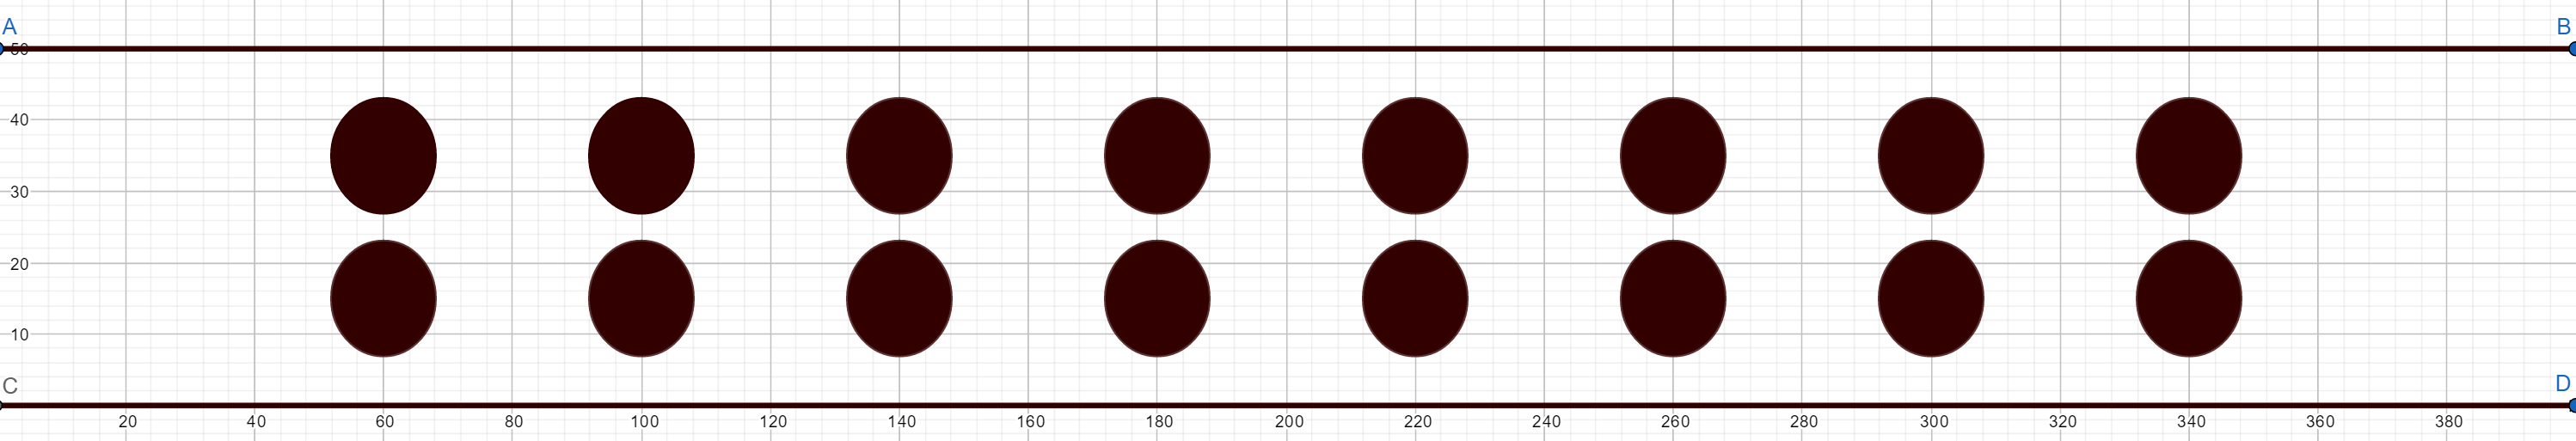
\includegraphics{Assets/MPCD_Pipe.png}
\caption{Container of MPCD fluid, with obstacles}
\end{figure}

\begin{figure}
\centering
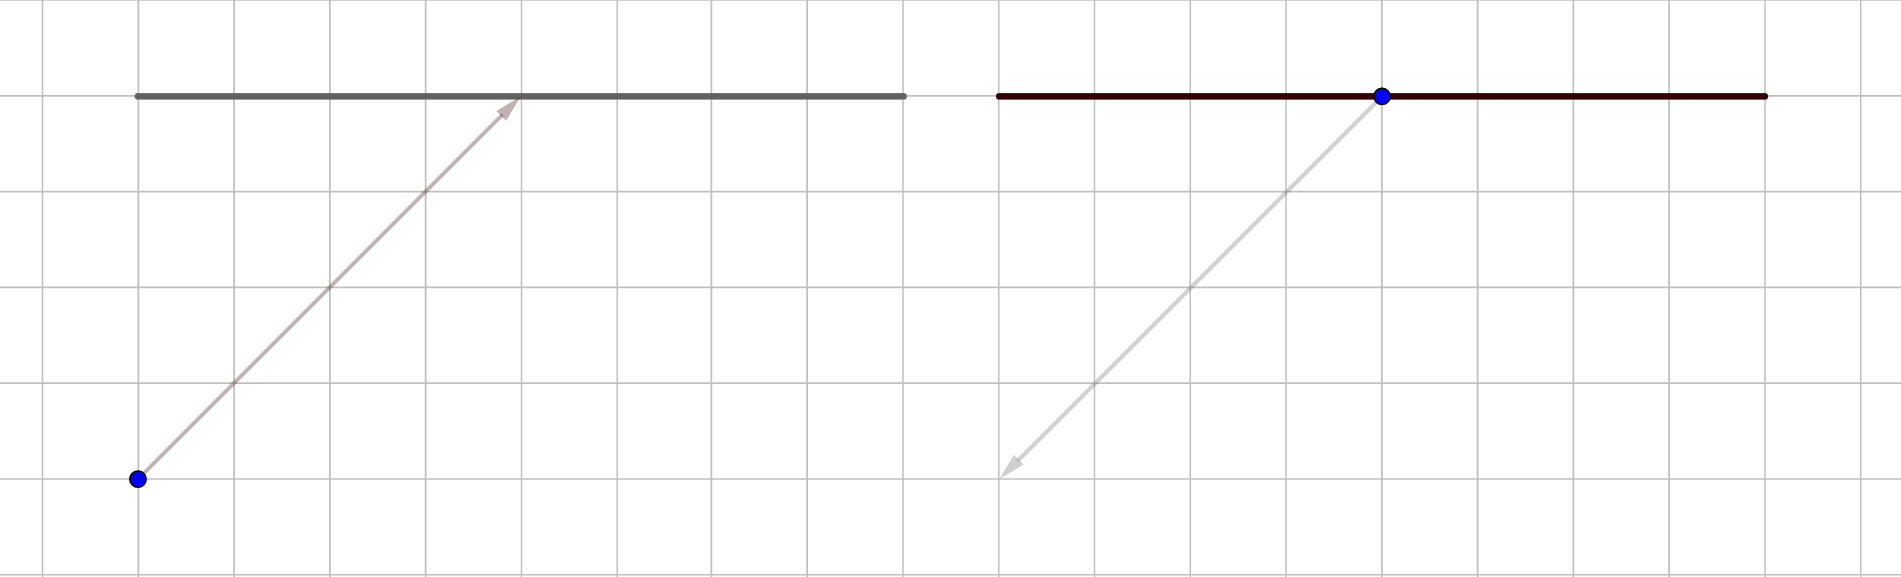
\includegraphics{Assets/Wall_stick_boundary_conditions_reflection.png}
\caption{Reflection of particle from wall, stick boundary conditions}
\end{figure}

Because of the shifting of the grid before the collision step, the cells
next to the walls might be partially blocked by the wall. This partial
blocking by the wall causes the cell to have, on average, less particles
than it would have, had the grid not been shifted. The change in average
particles distorts the collision step of particles near the wall. For
more complex geometries than the one used in this thesis, the wall wont
even be parallel to the grid lines, which makes this a problem even
without a grid shift. To compensate this, it has been shown in (TODO:
find a source) that the following process undoes the distortion.

As is shown in figure (TODO: figure numbering), imagine a cell being
blocked a little bit by the wall. Let's assume that the average number
of particles per cell is 4. In the first cell, we count 3 particles.
What is now done, is to introduce a ``virtual'' particle, which we might
imagine as being behind the wall, though the position of it does not
matter. Jumping to the second cell, we introduce 2 ``virtual
particles''. In general, \(\bar N_c - N_c\) particles are introduced,
where \(\bar N_c\) is the average number of particles per cell, chosen
to be an integer, and \(N_c\) is the actual number of particles found in
cell \(c\). Their velocities are sampled from two independent normal
distributions with mean \(\mu = 0\) and variation
\(\sigma^2 = \frac{k_{B}T}{m}\), where \(k_{B}\) is the boltzmann
constant, \(T\) is the temperature of the fluid, and \(m\) is the mass
of one particle.

\begin{figure}
\centering
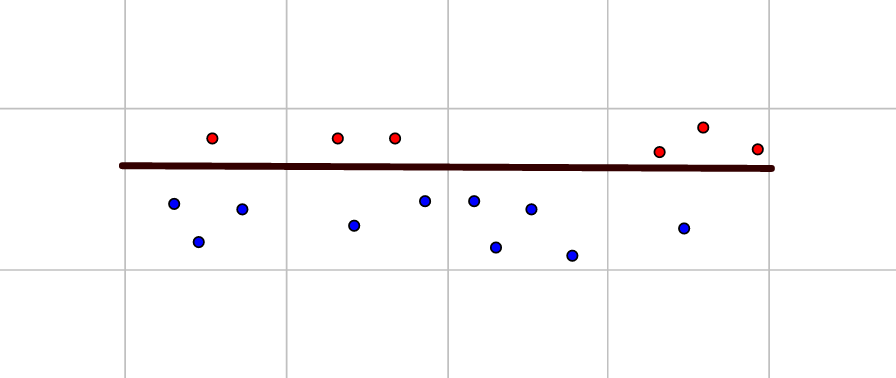
\includegraphics{Assets/Wall_stick_boundary_conditions_virtual_particles.png}
\caption{Undoing the distortion caused by the grid shift}
\end{figure}

\hypertarget{the-ballistics-step}{%
\subsection{The ballistics step}\label{the-ballistics-step}}

The ballistics step might be called a substep of particle streaming.
After the particles are moved, their position is checked for interaction
with the wall or obstacles. If particles overshoot the bounds set by
either the wall or obstacles, their position is set to the collision
point, their velocity is reversed, subsequently they are moved for the
rest of the distance they would have travelled, as explained in section.
(TODO: section numbering) This means we are assuming elastic collision
between the particles, the walls and obstacles.

\hypertarget{constant-force}{%
\subsection{Constant Force}\label{constant-force}}

Several methods exist to model poseuille flow. Here, a gravitational
approach is chosen. This means an external force acts on the unit volume
of the fluid, which is given by,

\begin{equation}
\vec{F} = \rho_S g \hat x,
\end{equation}

where \(\rho_S\) is the mass density of the solvent, \(g\) is the
acceleration constant and \(\hat x\) is the unit vector in the
\(x\)-direction. This force is incorporated into the simulation by
updating the position and velocity of a particle according to the
solution for constant force Newton's equations.(Nikoubashman et al.,
2013)

Because now a force acts on the particles, as seen in figure (TODO
figure\#), additional energy is coming into the system which needs to be
controlled. The tool to do this in MPCD is called a thermostat.

\begin{figure}
\centering
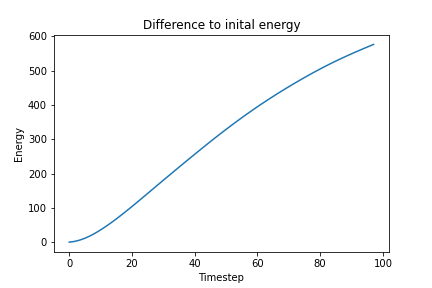
\includegraphics{Release/Assets/increasing_energy.png}
\caption{Increasing energy of system. Difference in energy at timestep t
vs.~t=0}
\end{figure}

\hypertarget{thermostat}{%
\subsection{Thermostat}\label{thermostat}}

To counteract the heating up of the fluid by the constant force on every
particle, a thermostat is needed. As described in Winkler(Gompper et
al., 2009), the computationally efficient cell-level thermostat was
used. For this, the macroscopic flow profile is needed. Fluid flow
through the cross section of a pipe with parallel walls and interaction
modeled by no-slip boundary condition is called poseuille flow, the
macroscopic flow profile is known. It is calculated as,

\begin{equation}
u(r) = \frac{\Delta p}{4\eta L_x} (R^2 - r^2),
\end{equation}

where \(u\) is the macroscopic velocity in the x-direction, \(\Delta p\)
is the difference in pressure from beginning to end of the pipe,
\(\eta\) is the dynamic viscosity of the fluid, \(L_x\) is the length of
the pipe, \(R\) is the radius of the pipe and \(r\) is the
\(y\)-coordinate of the particle relative to the center of the
pipe.(Wikipedia contributors, 2020c) The situation is displayed in
figure (TODO: make a figure)

TODO: The pressure difference is on the order of \(\Delta p \sim g\),
where g is the acceleration constant of the force.(Nikoubashman et al.,
2013) END TODO

TODO: The dynamic viscosity of water at body temperature is about
\(\eta \sim 0.6947\). END TODO

\hypertarget{anything-else-maybe}{%
\subsection{Anything else maybe ??}\label{anything-else-maybe}}

\hypertarget{implementing-the-mpcd-algorithm}{%
\section{Implementing the MPCD
Algorithm}\label{implementing-the-mpcd-algorithm}}

\hypertarget{random-number-generation}{%
\subsection{Random Number Generation}\label{random-number-generation}}

\hypertarget{uniform-random-number-generation}{%
\subsubsection{Uniform random number
generation}\label{uniform-random-number-generation}}

\emph{This section was shortened considerably. The old version can still
be found at the end of this report.}

Sampling numbers from a uniform distribution is very important for MPCD.
Even if we did not initialize positions randomly, but for example all at
one point, arguing that after a sufficient amount of timesteps, the
particles will spread out, the rotation angle still truly needs to be
random, in a statistical sense.

To this end, the xoshiro256++, developed by Sebastian Vigna and David
Blackman, was used. It is a fast algorithm that does well on a variety
of statistical tests. The xoshiro256++ belongs to the Xoshiro
algorithms, which are an extended variant of xorshift algorithms.(Vigna,
2019) Xoshiro stands for ``Xor, Shift, Rotation'' and xorshift stands
for ``Xor, Shift''. The Xoshiro algorithms, additional to xor and
bit-shift operations, incorporate bitrotation.(Vigna, Sebastiano,
2020)(Wikipedia contributors, 2020g)

\hypertarget{sampling-from-a-normal-distribution}{%
\subsubsection{Sampling from a normal
distribution}\label{sampling-from-a-normal-distribution}}

To initialize the velocities of generated particles, a Maxwell-Boltzmann
distribution must be used. In two, as well as in three dimensions, this
is equivalent to the product of two, or three, independent normal
distributions with mean \(\mu = 0\) and variance
\(\sigma^2 = \frac{k_{B}T}{m}\), where \(k_{B}\) is the boltzmann
constant, \(T\) is the temperature of the fluid, and \(m\) is the mass
of one particle. Thus, the velocities are sampled from normal
distributions.(Wikipedia contributors, 2020d)

For this purpose, the normal distribution of the C++ standard library
was used, along with a Mersenne Twister number generator, which,
although it has some shortcomings, will for all practical purposes
suffice for the scope of this thesis. Although the Xoshiro is far
superior to the Mersenne Twister algorithm(Vigna, 2019), to adapt it for
this purpose did not seem worth the effort, because the difference in
quality will not be visible.

\hypertarget{mpcd-barebones-algorithm}{%
\subsection{MPCD barebones algorithm}\label{mpcd-barebones-algorithm}}

\hypertarget{the-streaming-step-1}{%
\subsubsection{The streaming step}\label{the-streaming-step-1}}

\emph{This section was shortened, since I think it does not deserve its
own.}

The streaming step was implemented and tested in an older version of
this thesis.

\hypertarget{the-collision-step-1}{%
\subsubsection{The collision step}\label{the-collision-step-1}}

To model the interaction of particles with each other, we implement the
collision rules, as detailed in section (TODO: section numbering). To
avoid some of the downfalls of the original algorithm, as detailed in
section (TODO: section\#), we implement a grid shift.

\hypertarget{grid-shift}{%
\paragraph{Grid shift}\label{grid-shift}}

After particle streaming, the grid is shifted. The components of this
shift, \(\vec{s}\) are sampled from a uniform random distribution in the
interval \([-\frac{a}{2},\frac{a}{2}]\). This step is necessary to
restore Galilean invariance, which is violated when the molecular chaos
assumption does not hold. This happens when simulating cold fluids or
when using very small timesteps.(Ihle \& Kroll, 2001) The shift is
undone at the end of the collision step, after the velocity of all
particles has been updated.

If particles go out of the simulation bounds due to the grid shift, they
reappear at the other end as described in section (TODO: section
numbering). Because the wall will not align with the grid anymore,
virtual particles as described in section (TODO: section numbering) have
to be introduced.

\hypertarget{velocity-updating}{%
\paragraph{Velocity updating}\label{velocity-updating}}

\emph{TODO} \emph{Note: The floor is not rendering correctly at the
moment, but it's a mistake that will be fixed in the final version.}

The velocities of the particles update according to equation (TODO:
numbering equ). To calculate the mean velocity \(\vec{V_{c}}\) of cell
\(c\), first a way to assign each particle a cell has to be established.
Let the indices of the cell be \((i, j)\). The position of a cell can
then be calculated as \(x_c = j \cdot a + s_x\) and
\(y_c = i \cdot a + s_y\), where \(a\) is the lattice constant, \(s_x\)
and \(s_y\) are the \(x\) and \(y\) components of grid shift
\(\vec{s}\). So for the indices it follows,

\begin{equation}
i = floor{\frac{y - s_y}{a}}\\
j = floor{\frac{x - s_x}{a}},
\end{equation} where \((x,y)\) refers to the components of the
particle's position vector. With this method to determine the cells, the
total cell velocities and numbers of particles in each cell are
calculated to obtain the mean cell velocity. Using a uniform randomly
sampled rotation angle \(\alpha\) and rule (TODO: numbering equ), the
particles' velocities are updated.

\hypertarget{testing-mpcd-barebones}{%
\subsubsection{Testing MPCD barebones}\label{testing-mpcd-barebones}}

Having implemented the essential features of the MPCD algorithm, namely
the streaming and collision steps, it is time for testing it to make
sure it was implemented correctly. This section will present
conservation tests and visual tests. Note that there are no walls and no
obstacles, no forces and no thermostat, yet.

\hypertarget{timestep-animation}{%
\paragraph{Timestep animation}\label{timestep-animation}}

To inspect and understand the behavior of our simulation, an animation
was created. The fluid starts out in a random state, which means that
the positions and velocities of the particles are initialized randomly.

The initial state, and the one after 100 timesteps, of region
\(x \in (200, 240)\), \(y \in (0, 20)\) can be seen below (TODO
figure\#).

\textbf{An explanation of the plots}: Top left is a quiver plot, where I
plot the velocity vectors of cells at their position. Top right is
streamplot, where this same data is used to visualize streaming,
background work (interpolation, probably) done by python. Bottom left
are the particles positions in a 2d plane. Bottom right is a heatmap of
number of particles per cell (will be helpful when implementing walls,
because it should be less there if we don't implement virtual particles)

\emph{The animations were sent by mail. If you did not get them and
would like to see them, you can access them here:
https://www.dropbox.com/sh/ih11zkpzapvd7qm/AADgbdW\_ejXumRROJbCgMxaUa?dl=0}

\emph{The animations will probably be more interesting once force,
thermostat \& obstacles have been implemented, but it was a good way to
check the behavior of the simulation against the intuition.}

\begin{verbatim}
Loading particles ..
--loaded 10
--loaded 20
--loaded 30
--loaded 40
--loaded 50
--loaded 60
--loaded 70
--loaded 80
--loaded 90
--loaded 100
Particles loaded and saved!





Loading cells
--loaded 10
--loaded 20
--loaded 30
--loaded 40
--loaded 50
--loaded 60
--loaded 70
--loaded 80
--loaded 90
--loaded 100
Cells loaded and saved!

Preparing cell values ..
Cell preparation complete!




Plotting data ..
Data plotted and saved!
\end{verbatim}

\begin{figure}
\centering
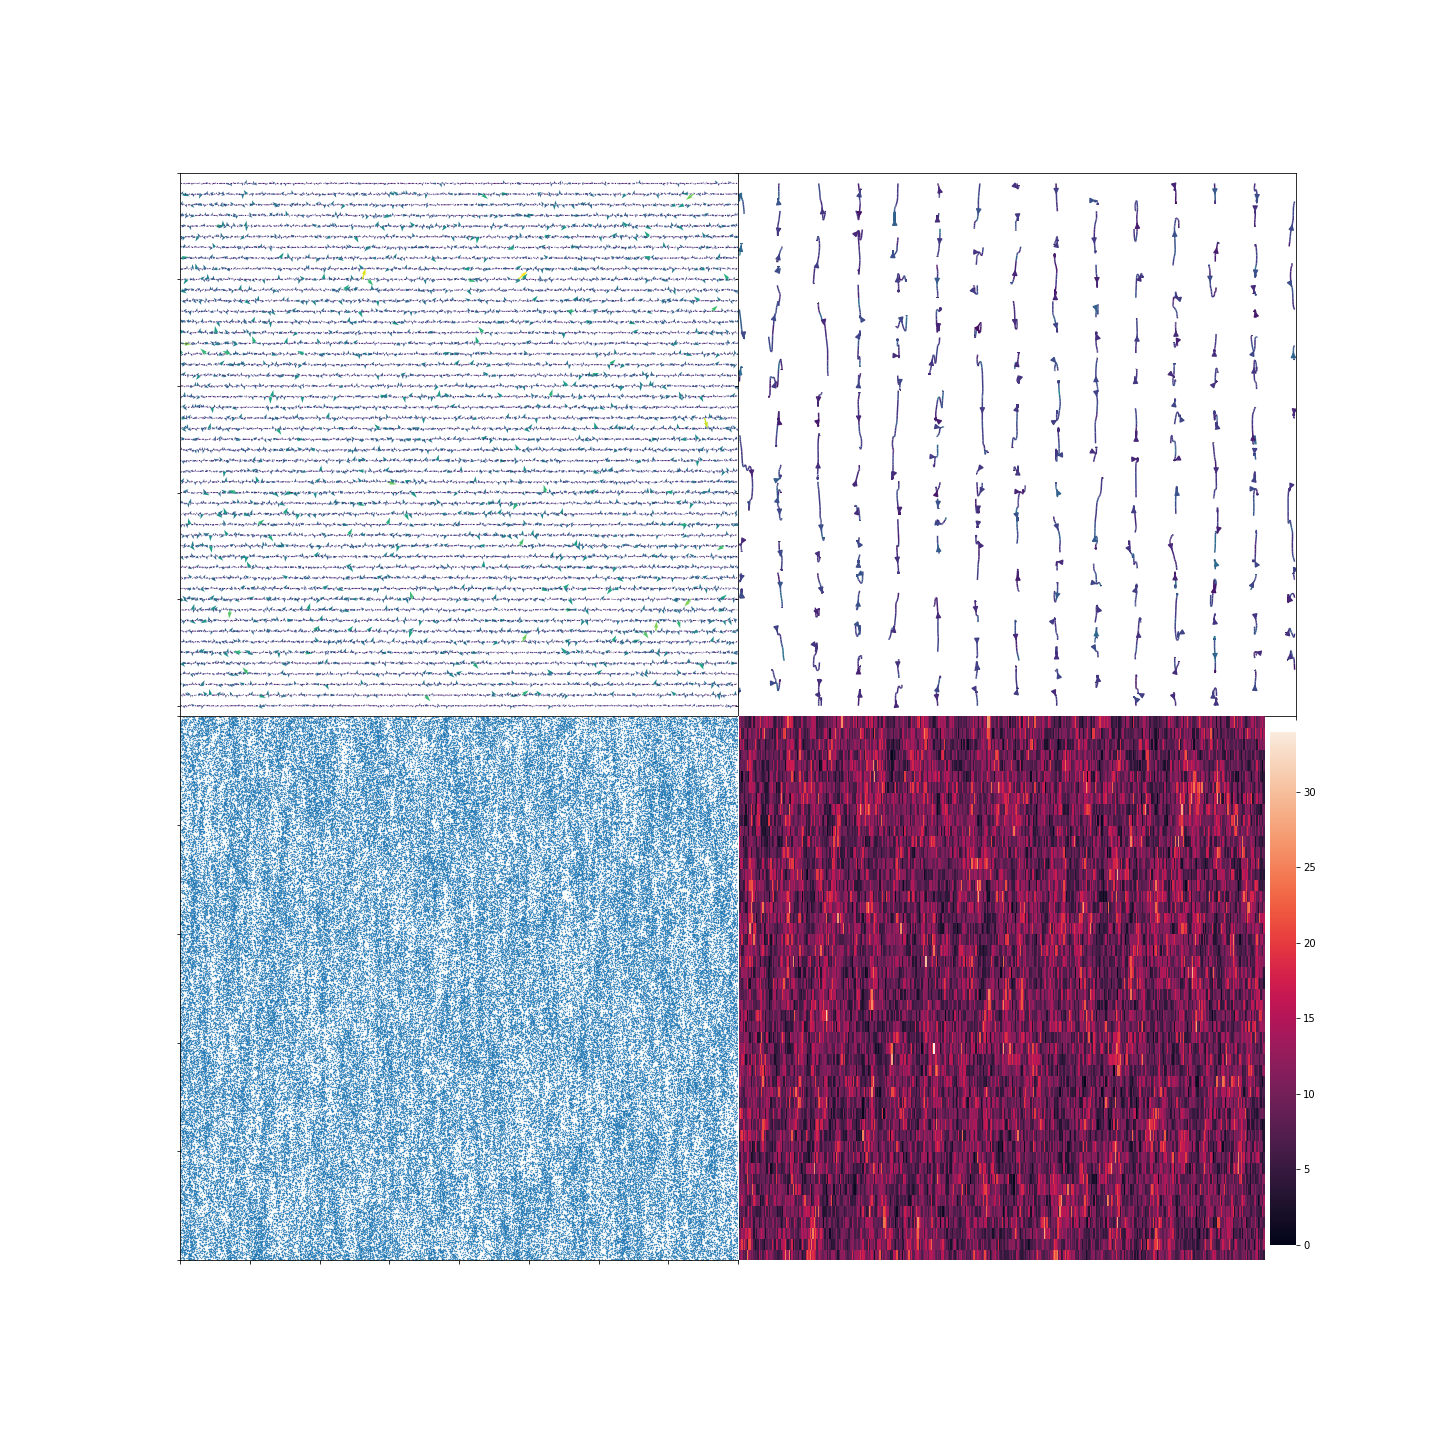
\includegraphics{Assets/initial_region.png}
\caption{Initial State of region with barebones MPCD implementation}
\end{figure}

\begin{verbatim}
Plotting data ..
Data plotted and saved!
\end{verbatim}

\begin{figure}
\centering
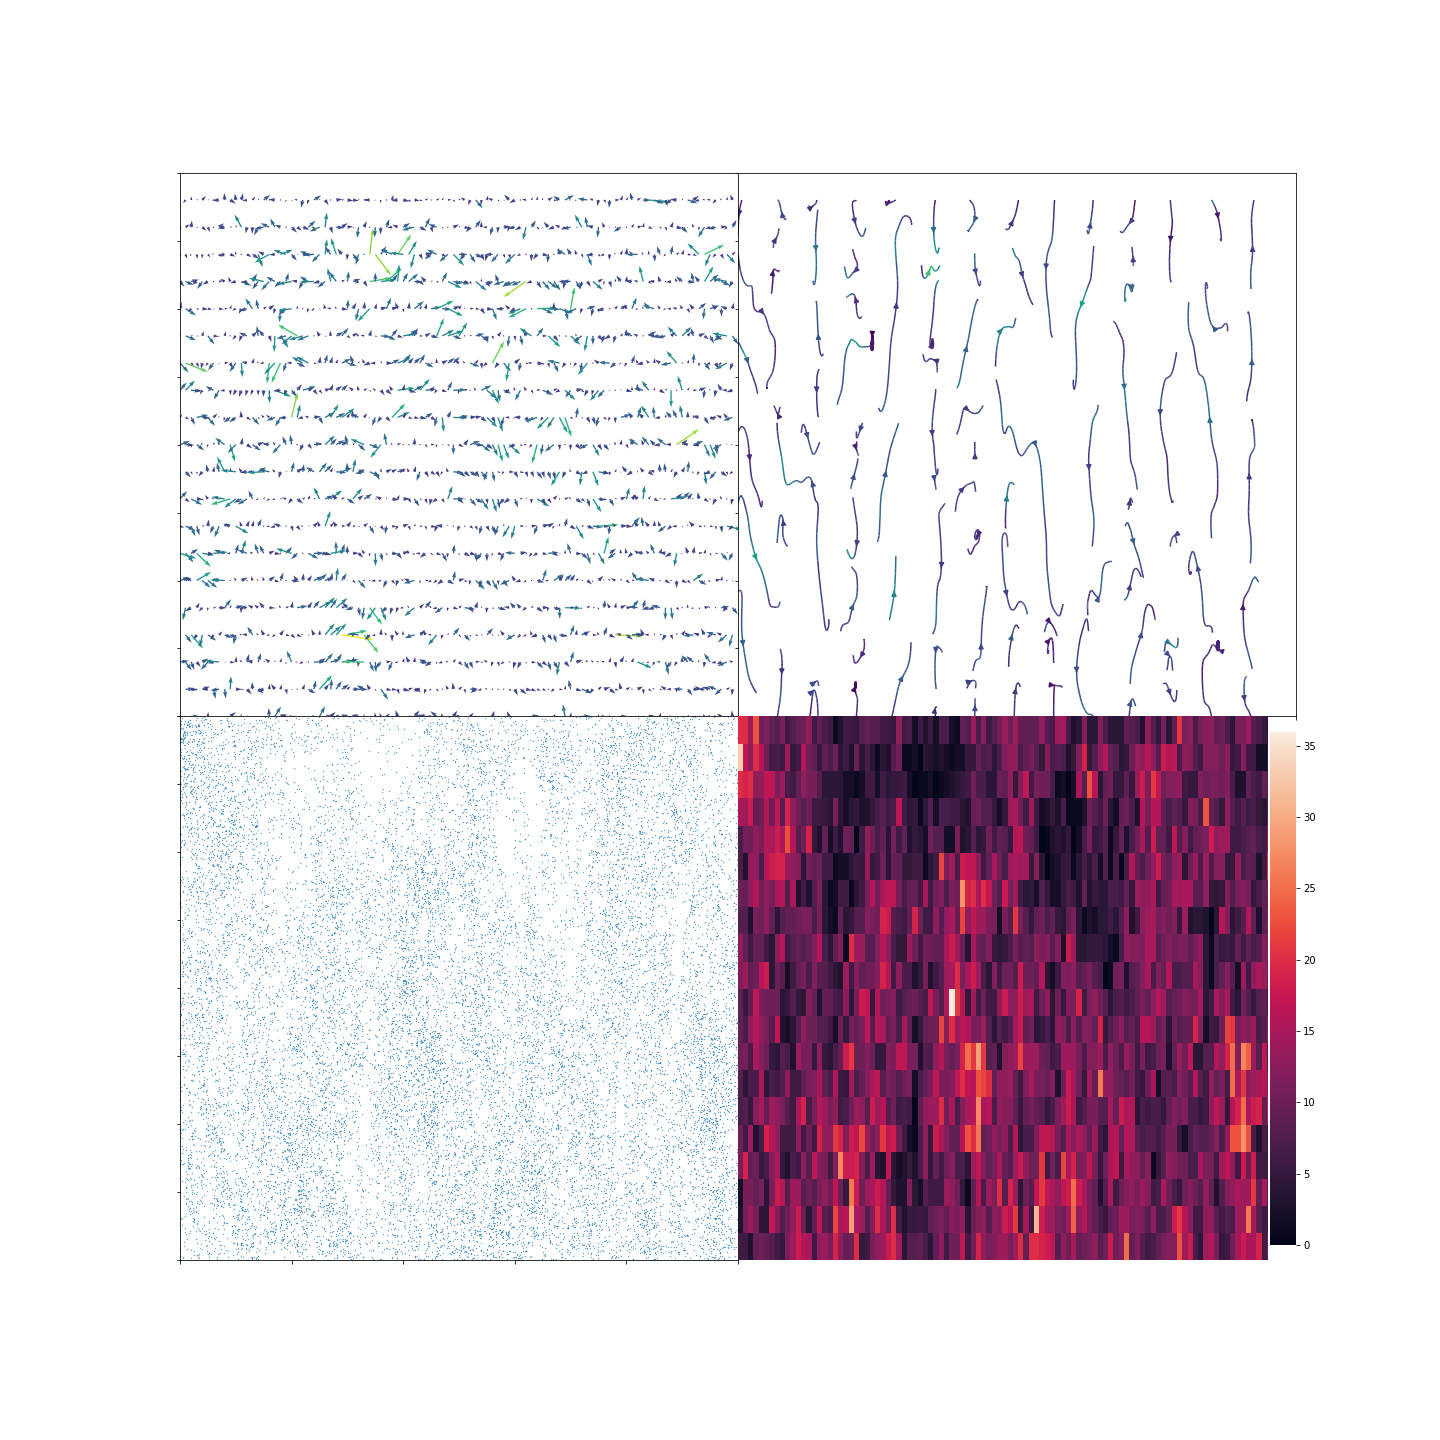
\includegraphics{Assets/stationary_region.png}
\caption{Ending (maybe stationary) state of region with barebones MPCD
implementation}
\end{figure}

\begin{verbatim}
Animating Quiver ...

--Created 0 frame.

--Created 0 frame.

--Created 10 frame.

--Created 20 frame.

--Created 30 frame.

--Created 40 frame.

--Created 50 frame.

--Created 60 frame.

--Created 70 frame.

--Created 80 frame.

--Created 90 frame.

Animated and saved!




Animating Streamplot ...

--Created 0 frame.

--Created 0 frame.

--Created 10 frame.

--Created 20 frame.

--Created 30 frame.

--Created 40 frame.

--Created 50 frame.

--Created 60 frame.

--Created 70 frame.

--Created 80 frame.

--Created 90 frame.
\end{verbatim}

\hypertarget{conservation-of-number-of-particles}{%
\paragraph{Conservation of number of
particles}\label{conservation-of-number-of-particles}}

The number of particles is (just for convenience) plotted and it stays
constant.

\begin{figure}
\centering
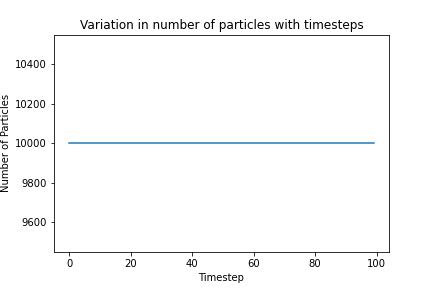
\includegraphics{Assets/number_particles.png}
\caption{Constant number of particles}
\end{figure}

\hypertarget{conservation-of-momentum}{%
\paragraph{Conservation of momentum}\label{conservation-of-momentum}}

Because the angle of rotation in the collision step is chosen randomly,
and the streaming step does not change momentum, in a large system
momentum should be conserved. The velocities of particles were taken and
added up. The base momentum is the initial momentum, the error (or
variation) from this base is plotted below.

\begin{figure}
\centering
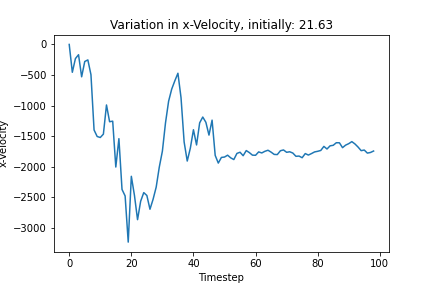
\includegraphics{Assets/x_velocity_variation.png}
\caption{Variation in x-velocity throughout simulation}
\end{figure}

\begin{figure}
\centering
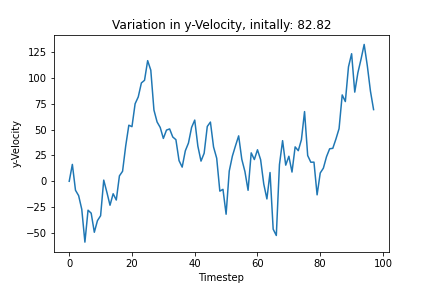
\includegraphics{Assets/y_velocity_variation.png}
\caption{Variation in y-velocity throughout simulation}
\end{figure}

\begin{figure}
\centering
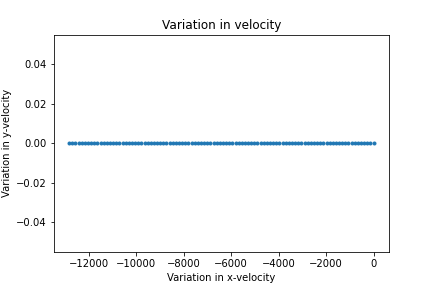
\includegraphics{Assets/velocity_variation.png}
\caption{Variation in velocity throughout simulation}
\end{figure}

Error \(\sim 10^{-5}\)

\hypertarget{energy}{%
\paragraph{Energy}\label{energy}}

The collision step of the MPCD algorithm conserves energy
\emph{locally}, which is to say on a cell level. (Gompper et al., 2009)
The energy should also be conserved globally, since no force is acting
upon the particles \emph{yet}, the streaming and collision steps
conserve energy, and the particle number remains the same.

To inspect this, the energy of every particle is added up. The base
energy is the initial energy, the error (or variation from this base) is
calculated and plotted below.

\begin{figure}
\centering
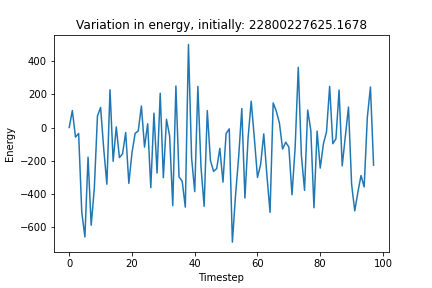
\includegraphics{Assets/constant_energy.png}
\caption{Constant energy throughout simulation}
\end{figure}

Error \(\sim 10^{-8}\)

\hypertarget{old-sections-or-not-fitting}{%
\section{Old sections, or not
fitting}\label{old-sections-or-not-fitting}}

\hypertarget{pseudo-random-number-generation}{%
\subsection{(Pseudo) Random Number
Generation}\label{pseudo-random-number-generation}}

\hypertarget{sampling-from-uniform-distribution}{%
\subsubsection{Sampling from uniform
distribution}\label{sampling-from-uniform-distribution}}

One of the pillars of this thesis is the generation of random rotation
angles for the rotation matrix needed in the collision step. This proved
to be somewhat difficult. First, the standard algorithm of the C++
standard library was tried, but it didn't qualify because it performed
poorly in comparison to the second and third algorithms tried, which are
called ``Mersenne Twister'' and ``xoshiro256++'',
respectively.(Wikipedia contributors, 2020e)(cppreference contributors,
2020)(Vigna, Sebastiano, 2020)

The Mersenne Twister was implemented using the C++ standard library. The
xoshiro256++ was implemented using Sebastian Vigna's code with some
additions.(Vigna, Sebastiano, 2020)

To compare algorithms, and also to make sure that the implementation of
the xoshiro256++ is right, a \(\chi^2\) test for discrete observations
was used. The generated angles in the interval \([0, 2\pi)\) were split
into \(k+1\) buckets, where \(k\) is the number of degrees of freedom of
the \(\chi^2\) distribution. The test error

\begin{equation}
T = \sum_{b=1}^{k+1}{\frac{(N_o - E[N_b])^2}{E[N_b]}},
\end{equation}

where \(E[N_b] = \frac{N}{b}, b \in \{1, 2, \dots , k+1\}\) is the
expected bucket size, is compared to \(\chi^2_{1-\alpha, k}\), where
\(\alpha\) is the signifigance level. The null hypothesis

\[
H_0: \textrm{The angles are distributed uniformly in the interval } [0, 2 \pi)
\]

is tested against the alternative hypothesis

\[
H_1: \textrm{The angles are not distributed uniformly in the interval } [0, 2 \pi) \textrm{.}
\]

If the test should have significance level \(\alpha\), \(H_0\) is
rejected if \(T \ge \chi^2_{1-\alpha, k}\).(Frühwirth, Rudolf,
n.d.)(Wikipedia contributors, 2020a)(Wikipedia contributors, 2020b)

The results of the \(\chi^2\) test are summarised in {[}TODO: Table, and
table formatting{]}.

As we can see, both generators pass the \(\chi^2\) test and we do not
have to reject our null hypothesis \(H_0\).

Visually, we can examine the generated buckets of both random generators
in {[}TODO{]} the following plot.

\begin{figure}
\centering
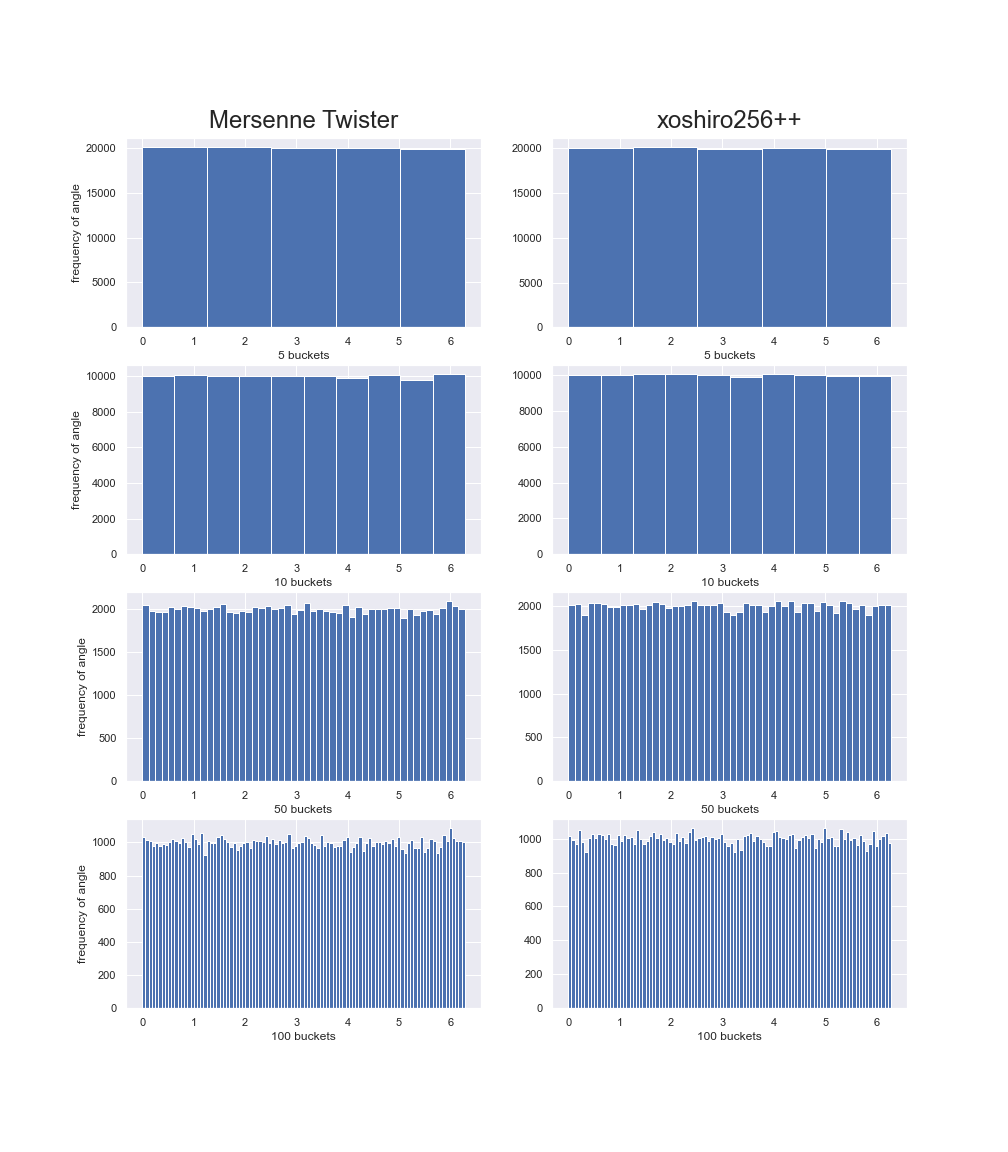
\includegraphics{Assets/angle_buckets.png}
\caption{A histogram of different bucket sizes generated by MT and
xoshiro256++}
\end{figure}

The Mersenne Twister has been known to fail certain statistical tests
since its inception, by virtue of its mathematical characteristics.
There exist other algorithms that are designed to be faster and that do
not fail any known statistical tests, examples of which are almost all
of the algorithms in the xoshiro family.(Vigna, 2019) Ultimately, the
xoshiro256++, developed by Sebastian Vigna and David Blackman, was used.
It is a variant of the xorshift algorithm, which extends the bit-shift
and xor methods by bitrotation, making it still very fast, and more
``random'' than the xorshift.(Wikipedia contributors, 2020g)(Vigna,
Sebastiano, 2020)

Note that testing a (pseudo) random number generator is usually much
more involved than this, but since this has already been done
extensively by other authors, we are satisfied with the \(\chi^2\) test,
simply to test the implementation of the xoshiro256++, since it plays an
important part.(Wikipedia contributors, 2020f)(Vigna, 2019)

\hypertarget{grid}{%
\subsection{Grid}\label{grid}}

For the implementation of the collision step, a regular lattice is
needed.(Gompper et al., 2009) This grid has lattice constant \(a\),
which in this thesis will simply be \(1\). Each cell of the grid has an
average number of particles per cell, which is typically initialised to
between three and 20, although it can be as high as 70(Ihle \& Kroll,
2001). This number mainly affects the viscosity of the fluid.(TODO: find
source) The average number of particles for the studied situation is
\(\bar N_c = 10\).

TODO: update situation

\begin{figure}
\centering
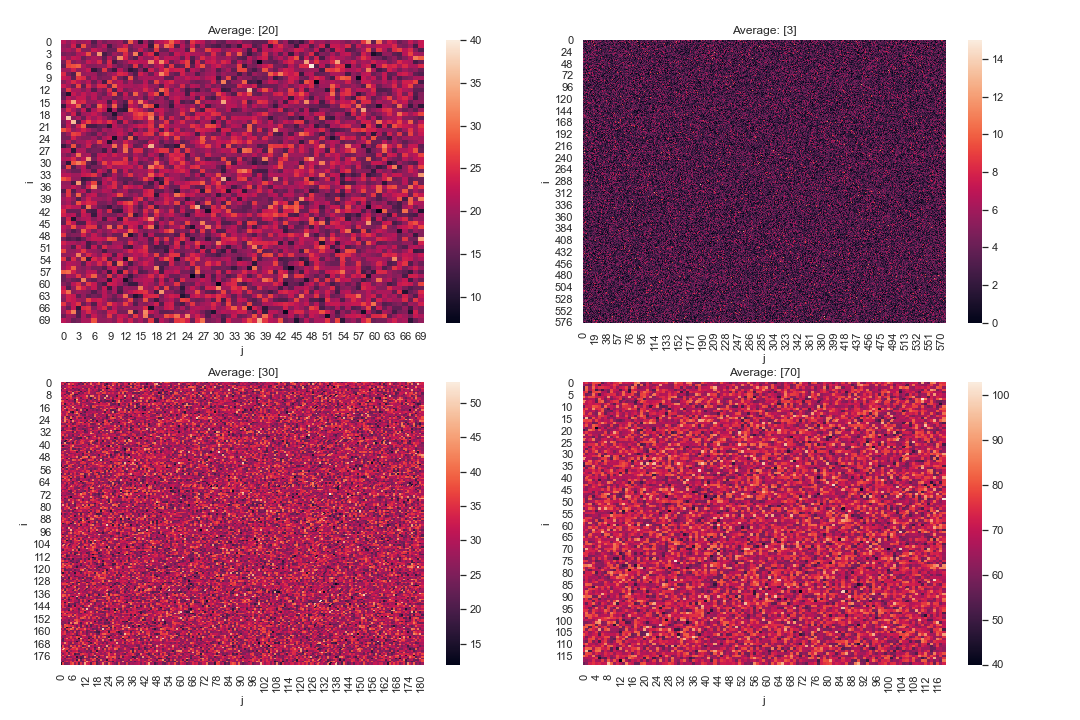
\includegraphics{Assets/average_grid_particles.png}
\caption{Average number of particles per Grid cell}
\end{figure}

\hypertarget{the-streaming-step-2}{%
\subsection{The streaming step}\label{the-streaming-step-2}}

The particle positions were drawn from a uniform real distribution in
the same interval as the dimensions of the pipe. The velocities were
sampled from a normal distribution as described in section (TODO:
section number) The results can be seen in figure {[}TODO: figure
numbering{]} below. From the positions in the first row, the velocities
in the second row, particle streaming is applied for 1 and 10 timesteps,
according to equation (TODO: equ numbering).

TODO: update situation

\begin{figure}
\centering
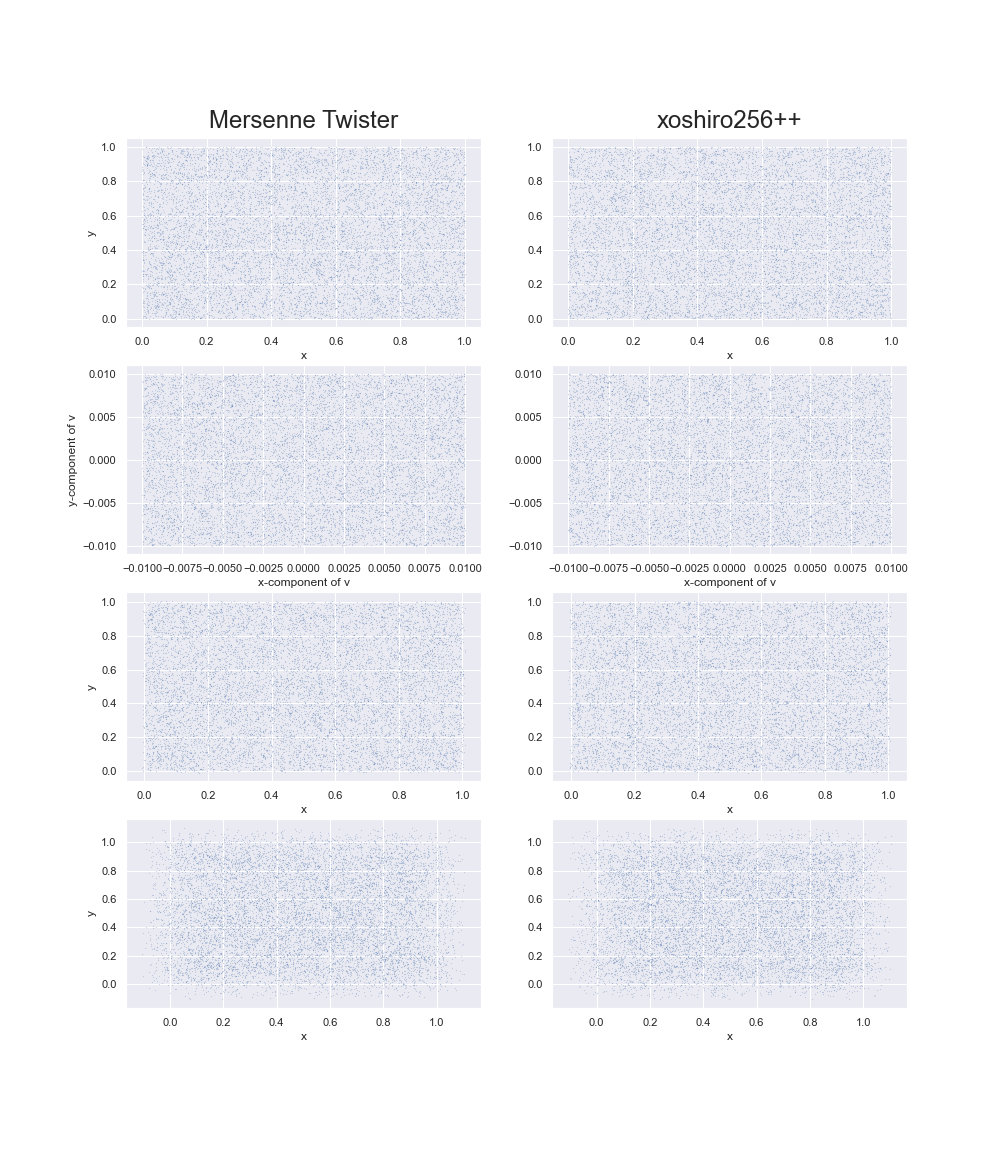
\includegraphics{Assets/particle_streaming.png}
\caption{Particle streaming without collision with MT and with xoshiro}
\end{figure}

We see the x and y coordinates are randomly initialized according to the
shape of the container. Looking closely, one can see that our particles
look very much like noise. The absolute value of the velocity components
are initialized to at most 1\% of their respective dimensions. After one
timestep, some of the particles on the outer ranges have moved out of
bounds, and after ten timesteps, the particles have thinned out
considerably along the edges.

\hypertarget{optimizing-the-algorithm}{%
\subsection{Optimizing the algorithm}\label{optimizing-the-algorithm}}

To optimize the runtime of the simulation, the code was analyzed for CPU
\& memory usage. Several areas were identified that needed improvement.
In the end, the streaming and collision step are now performed in
parallel, with the performance of the latter being very satisfying. The
performance of the streaming step however could not be optimized much
further. The problem is storage shared between threads, which means, to
prevent errors and undefinable behavior, the program can't make full use
of parallelization. It was tried to split this shared storage and later
recombine, but this was to no avail. Ultimately, a lot of time was spent
on this but unfortunately, the intricacies of C++ made this seem
impossible.

The reason a lot of time was spent on this particular step is to make
possible a larger simulation, i.e.~larger number of particles.

\hypertarget{refs}{}
\begin{cslreferences}
\leavevmode\hypertarget{ref-cppreference:prng}{}%
cppreference contributors. (2020). \emph{Pseudo-random number generation
- cppreference.com}.
\url{https://en.cppreference.com/w/cpp/numeric/random}

\leavevmode\hypertarget{ref-fruehwirthstat}{}%
Frühwirth, Rudolf. (n.d.). \emph{Wahrscheinlichkeitsrechnung und
Statistik}.

\leavevmode\hypertarget{ref-winkl2009}{}%
Gompper, G., Ihle, T., Kroll, D. M., \& Winkler, R. G. (2009).
Multi-Particle Collision Dynamics: A Particle-Based Mesoscale Simulation
Approach to the Hydrodynamics of Complex Fluids. In \emph{Advanced
computer simulation approaches for soft matter sciences iii} (Vol. 221,
p. 1). \url{https://doi.org/10.1007/978-3-540-87706-6_1}

\leavevmode\hypertarget{ref-ihlekroll2001}{}%
Ihle, T., \& Kroll, D. M. (2001). Stochastic rotation dynamics: A
galilean-invariant mesoscopic model for fluid flow. \emph{Phys. Rev. E},
\emph{63}(2), 020201. \url{https://doi.org/10.1103/PhysRevE.63.020201}

\leavevmode\hypertarget{ref-malev1999}{}%
Malevanets, A., \& Kapral, R. (1999). Mesoscopic model for solvent
dynamics. \emph{The Journal of Chemical Physics}, \emph{110}(17),
8605--8613.

\leavevmode\hypertarget{ref-nikoubashman2013}{}%
Nikoubashman, A., Likos, C. N., \& Kahl, G. (2013). Computer simulations
of colloidal particles under flow in microfluidic channels. \emph{Soft
Matter}, \emph{9}(9), 2603--2613.
\url{https://doi.org/10.1039/C2SM26727F}

\leavevmode\hypertarget{ref-vigna2019}{}%
Vigna, S. (2019). It is high time we let go of the Mersenne Twister.
\emph{arXiv E-Prints}, arXiv:1910.06437.
\url{http://arxiv.org/abs/1910.06437}

\leavevmode\hypertarget{ref-unimi:xoshiro}{}%
Vigna, Sebastiano. (2020). \emph{Xoshiro/xoroshiro generators and the
prng shootout}. \url{http://prng.di.unimi.it/}

\leavevmode\hypertarget{ref-wiki:chisquaredtest}{}%
Wikipedia contributors. (2020a). \emph{Chi-squared test --- Wikipedia,
the free encyclopedia}.
\url{https://en.wikipedia.org/w/index.php?title=Chi-squared_test\&oldid=968434424}.

\leavevmode\hypertarget{ref-wiki:goodnessoffit}{}%
Wikipedia contributors. (2020b). \emph{Goodness of fit --- Wikipedia,
the free encyclopedia}.
\url{https://en.wikipedia.org/w/index.php?title=Goodness_of_fit\&oldid=962081310}

\leavevmode\hypertarget{ref-wiki:poseuille_equation}{}%
Wikipedia contributors. (2020c). \emph{Hagen--poiseuille equation ---
Wikipedia, the free encyclopedia}.
\url{https://en.wikipedia.org/w/index.php?title=Hagen\%E2\%80\%93Poiseuille_equation\&oldid=975461486}

\leavevmode\hypertarget{ref-wiki:maxwell_boltzmann}{}%
Wikipedia contributors. (2020d). \emph{Maxwell--boltzmann distribution
--- Wikipedia, the free encyclopedia}.
\url{https://en.wikipedia.org/w/index.php?title=Maxwell\%E2\%80\%93Boltzmann_distribution\&oldid=978374316}

\leavevmode\hypertarget{ref-wiki:mersennetwister}{}%
Wikipedia contributors. (2020e). \emph{Mersenne twister --- Wikipedia,
the free encyclopedia}.
\url{https://en.wikipedia.org/w/index.php?title=Mersenne_Twister\&oldid=969551905}

\leavevmode\hypertarget{ref-wiki:prng}{}%
Wikipedia contributors. (2020f). \emph{Pseudorandom number generator ---
Wikipedia, the free encyclopedia}.
\url{https://en.wikipedia.org/w/index.php?title=Pseudorandom_number_generator\&oldid=959248716}.

\leavevmode\hypertarget{ref-wiki:xorshift}{}%
Wikipedia contributors. (2020g). \emph{Xorshift --- Wikipedia, the free
encyclopedia}.
\url{https://en.wikipedia.org/w/index.php?title=Xorshift\&oldid=967790330}.
\end{cslreferences}

\end{document}
